%!TEX root = ../../thesis.tex
\chapter{Modellierung und Implementation}
\label{cha:modelling}

\todo[inline]{Intro}

\section{Spezifikation der Anforderungen}
\label{sec:requirements}
Der zu entwerfende Simulator soll die Ausführung ausgewählter Garbage-Collection-Algorithmen demonstrieren, sodass die einzelnen Arbeitsschritte eines Algorithmus klar erkennbar sind.
Dazu soll das in Kapitel~\ref{cha:intro} eingeführte Speichermodell realisiert werden.
Eine grafische Ausgabe visualisiert dabei den Heap als Blockgrafik: Belegte Teile des Heaps sollen von freien optisch unterschieden werden können, zudem sollen Lage und Größe der einzelnen Objekte erkennbar sein.
Die Anwenderin soll darüber hinaus die Möglichkeit haben, den Simulator zu konfigurieren:
Neben einer obligatorischen Auswahl des verwendeten Garbage-Collection-Algorithmus soll auch die Größe des Heaps sowie die Größe der erzeugten Heapobjekte einstellbar sein.
Weitere Anpassungsmöglichkeiten sind der Verzweigungsgrad der Objekte untereinander sowie die Verwaisungswahrscheinlichkeit, sodass verschiedene Objektkonstellationen betrachtet werden können.
Zuletzt soll durch eine Anpassbarkeit der Animationsgeschwindigkeit auch die Visualisierung anpassbar sein.

Aus Sicht der Softwareentwicklung ergeben sich zusätzliche Anforderungen, die für die Umsetzung der Anwendung relevant sind:
Der Simulator soll als frei verwendbare Software im Rahmen der Lehre eingesetzt werden können und beliebig anpassbar und erweiterbar sein, etwa indem Entwicklerinnen weitere Garbage-Collection-Algorithmen ergänzen.
Dies impliziert die Verwendung verschiedener Konzepte der Objektorientierung, unter anderem der Modularisierung in funktional unterscheidbare Pakete und Klassen, der Polymorphie und der generischen Programmierung.
Darüber hinaus soll die Anwendung plattformunabhängig entwickelt werden, um sie möglichst vielen Anwenderinnen zugänglich zu machen.

\section{Modellierung}
\label{sec:model}
Aufgrund der oben beschriebenen Anforderungen bietet sich die in Abbildung~\ref{fig:model} dargestellte Aufteilung in einzelne Komponenten an, auf deren Funktion im Folgenden eingegangen wird.
Bereits in Kapitel~\ref{cha:intro} wurde angemerkt, dass sich ein Programm grob in die drei Bestandteile Mutator, Allokator und Kollektor einteilen lässt.
Insofern ist es sinnvoll, diese Einteilung möglichst auch in die Modellierung einfließen zu lassen, insbesondere um verschiedene Kombinationen von Allokator und Kollektor zu ermöglichen.

\begin{figure}[h]
	\centering
	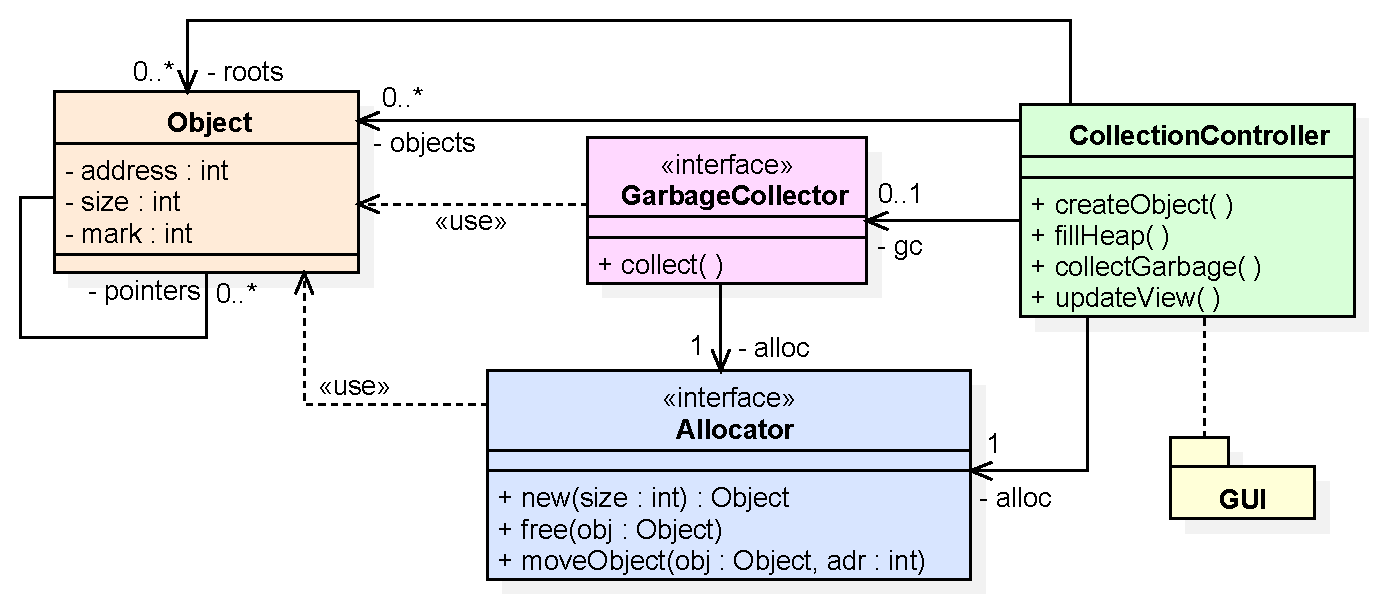
\includegraphics[scale=0.6]{img/uml/ch7-model.pdf}
	\caption[Klassendiagramm zur Modellierung von Mutator, Allokator und Kollektor]{Klassendiagramm zur Modellierung der Beziehung zwischen Mutator, Allokator und Kollektor. Im Rahmen der Implementation wurde dieses Modell um weitere Klassen, Methoden und Attribute ergänzt.}
	\label{fig:model}
\end{figure}

Heapobjekte werden als Instanzen einer Klasse \code{HeapObject} modelliert und beinhalten Speicheradresse (\code{address}), Größe (\code{size}), Markierungsinformation (\code{mark}) und eine Menge \code{pointers} an Referenzen auf weitere Instanzen von \code{HeapObject}, um die Menge \Pointers zu realisieren.
Ansonsten bieten sie keinerlei Funktionalität an.

Eine Instanz der Schnittstelle \code{Allocator} stellt die wesentlichen Dienste eines Allokators zu Verfügung.
Dazu zählt die Anforderung einer Speichermenge durch den Mutator mittels \code{new}, die Freigabe von Objekten und des durch sie belegten Speicherbereichs sowie das Verschieben eines Objekts.
Ersteres geschieht durch Übergabe der gewünschten Speichermenge und Rückgabe eines neu erzeugten Instanz von \code{HeapObject}, die die entsprechende Speicheradresse enthält.
Der Allokator ist diejenige Instanz, die Informationen über den Füllstand des Heaps und insbesondere über die Belegung einzelner Wörter besitzt.
Die Schnittstelle \code{GarbageCollector} beschreibt die Funktionalität eines Kollektors, welche im Wesentlichen aus der Durchführung eines Garbage-Collection-Zyklus (Methode \code{collect}) besteht.
Da eine Garbage Collection die Freigabe und Verschiebung von Objekten auslösen kann, verwaltet sie genau eine Instanz von \code{Allocator}.
Die Klasse \code{CollectionController} realisiert einerseits die Aufgabe des Mutators, das heißt die Anforderung von Speicher für neue Objekte sowie die (Simulation von) Referenzmanipulationen, die zur Verwaisung von Objekten führen.
Daher besitzt sie zwei Mengen von Heapobjekten \code{objects} und \code{roots}.
\code{objects} enthält dabei sämtliche Objekte des Heaps und \code{roots}\ -- entsprechend der Menge \Roots -- alle Basisobjekte.
Zudem verwaltet sie eine \code{Allocator}-Instanz, um Speicher anfordern zu können, sowie eine \code{GarbageCollector}-Instanz zur Auslösung der Garbage Collection.
Andererseits fungiert \code{CollectionController} als Steuerklasse, um über die GUI eingehende Benutzerinteraktionen umsetzen und delegieren zu können.

Die Idee ist nun, beim Start des Simulators zunächst eine Instanz der Klasse \code{CollectionController} erzeugen.
Diese legt wiederum -- je nach ausgewählter Garbage Collection -- eine geeignete \code{Allocator}-Instanz sowie einen \code{GarbageCollector} an.
Letzterer bekommt dabei den zuvor erzeugten Allokator übergeben, sodass Kollektor und Steuerklasse auf denselben simulierten Heap zugreifen.

\section{Implementation}
\label{sec:implementation}
Im nun folgenden Abschnitt wird vorgestellt, wie die obige Modellierung unter Beachtung der spezifizierten Anforderungen realisiert werden.
Im Sinne der Plattformunabhängigkeit wurde dazu die Programmiersprache \textit{Java} gewählt, wobei auf die \textit{Java Language Specification 9}\footnote{\url{https://docs.oracle.com/javase/specs/jls/se9/html/index.html}} zurückgegriffen wird.
Der gesamte Programmcode wurde über das Versionskontrollsystem \textit{Git}\footnote{\url{https://git-scm.com/}} verwaltet.
Um eine plattformunabhängige Entwicklung zu gewährleisten, wurde zudem das Build-Management-Tool \textit{Apache Maven}\footnote{\url{https://maven.apache.org/}} verwendet.
Dieses bildet die verschiedenen Arbeitsschritte der Entwicklung, wie etwa Kompilieren, Testen und Erzeugen von \code{JAR}-Dateien, auf automatisiert durchführbare Phasen ab und kümmert sich dabei eigenständig um Abhängigkeiten von externen Bibliotheken.
Zur Weiterentwicklung des Systems genügt somit ein Klonen des Git-Repositorys und eine Ausführung von Maven, um alle benötigten Abhängigkeiten beschaffen zu lassen.

Bei der Entwicklung der einzelnen Komponenten wurde grundsätzlich \textit{testgetrieben} vorgegangen.
Das bedeutet, dass zu jeder zu implementierenden Methode zunächst mehrere Testfälle erstellt werden, die das erwartete Verhalten des Programms beschreiben.
Einzige Ausnahme bilden hier Methoden, die mit GUI-Komponenten interagieren, da diese nur schwer automatisiert testbar sind.
Als Testframework wurde auf \textit{JUnit 5}\footnote{\url{https://junit.org/junit5/}} zurückgegriffen.

\newpage

\begin{figure}[H]
	\centering
	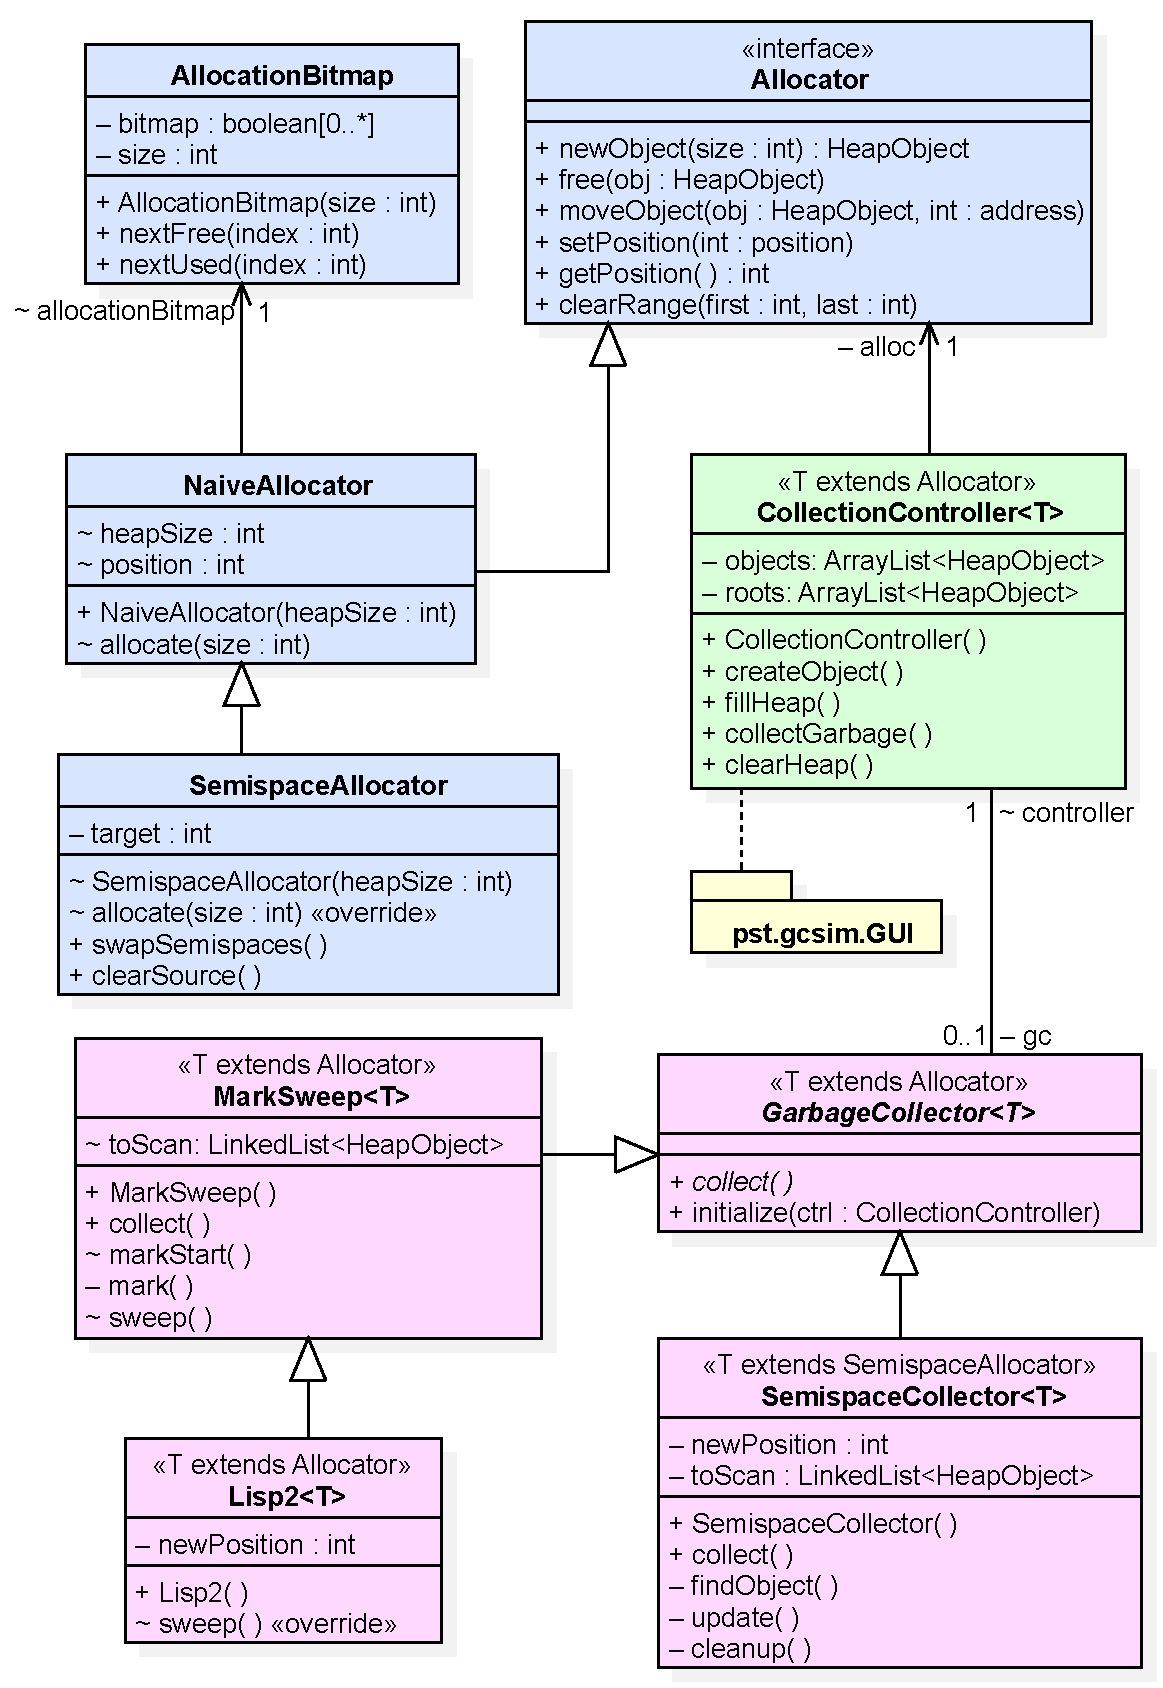
\includegraphics[scale=0.65]{img/uml/ch7-klassen.pdf}
	\caption[Klassendiagramm des realisierten Modells (Auszug)]{Klassendiagramm (Auszug) des realisierten Modells aus Abbildung~\ref{fig:model}.}
	\label{fig:implementation}
\end{figure}

\subsection{Allokator}
\label{sub:allocator}
Der Allokator verwaltet die Information, welche Wörter des simulierten Heaps belegt sind.
Aus diesem Grund wurde zunächst eine Klasse \code{AllocationBitmap} entworfen, die diese Information in einem \mintinline{java}{boolean}-Array speichert (siehe Abbildung~\ref{fig:implementation}).
Der $i$-te Eintrag dieses Arrays gibt an, ob das $i$-te Wort des Heaps durch ein Wort belegt (\mintinline{java}{true}) oder frei (\mintinline{java}{false}) ist.
Weiter stellt \code{AllocationBitmap} zwei Methoden \code{nextFree} und \code{nextUsed} zur Verfügung, welche ausgehend von einer übergebenen Speicheradresse die nächste freie bzw. belegte Stelle des Heaps liefern, indem das Array linear durchsucht wird.
Diese Methoden sind essenziell, um für eine angeforderte Speichermenge eine hinreichend große freie Stelle zu finden.

Als Konkretisierung der Schnittstelle \code{Allocator} wurde zunächst ein naiver Allokator entwickelt.
Dieser zeichnet sich dadurch aus, dass er -- ausgehend von einer Startposition -- mittels linearer Traversierung die nächstbeste freie Stelle findet, die die angeforderte Speichermenge aufnehmen kann.
Die Startposition ist dabei gegeben durch das Attribut \code{position}, welches stets die Adresse des ersten Worts hinter dem zuletzt angelegten Objekt enthält.

Das Herzstück der Klasse \code{NaiveAllocator} ist die Methode \code{allocate}, die intern durch \code{newObject} aufgerufen wird und das Auffinden einer geeigneten Position für ein neues Heapobjekt übernimmt (siehe Listing~\ref{java:naive-alloc}).
Diese Methode sucht zunächst unter Zuhilfenahme von \code{nextFree} und \code{nextUsed} der Reihe nach alle freien Stellen hinter \code{position} ab, bis eine genügend große gefunden oder das Ende des Heaps erreicht wurde (Zeile~7 bis~14).
Dabei wird auch berücksichtigt, dass sich hinter \code{position} eventuell kein freier Speicher befindet (Zeile~9f) oder ein freie Speicherbereich sich bis ans Heapende erstreckt (Zeile 12f).
Wird so ein hinreichend großer Bereich freien Speichers gefunden, wird dieser entsprechend der angeforderten Speichermenge als belegt markiert und die Anfangsadresse des Bereichs zurückgegeben (Zeile~18 bis 22).
Andernfalls wird auf analoge Weise der Bereich vor \code{position} durchsucht.
Sollte auch hierbei kein geeigneter Speicherbereich gefunden werden können, wird als Ergebnis \code{-1} zurückgegeben, was \code{newObject} dazu veranlasst, kein neues Objekt zu erzeugen.

\begin{listing}[h]
\inputminted[]{java}{code/NaiveAlloc-allocate.java}
\caption[Methode \code{allocate} der Klasse \code{NaiveAllocator}]{Auszug aus der Methode \code{allocate} der Klasse \code{NaiveAllocator}.}
\label{java:naive-alloc}
\end{listing}

Der \code{SemispaceAllocator} wurde zur Realisierung des Halbraumverfahrens nach \textsc{Fenichel}, \textsc{Yochelson} und \textsc{Cheney} (siehe Abschnitt~\ref{sec:copying}) entwickelt.
Die Allokation läuft hier weitestgehend analog zum \code{NaiveAllocator} ab, allerdings wird der Allokationsversuch auf den aktuellen Zielhalbraum beschränkt, dessen Beginn im Attribut \code{target} notiert ist.
Zusätzlich steht eine Methode \code{swapSemispaces} zur Verfügung, die die Rolle der beiden Halbräume tauscht, sowie eine Methode \code{clearSource}, die einen Halbraum in Gänze als unbelegt markiert.